
We would like to generalize the sorting problem. What if, when sorting a set of
elements, we already had some information on the order of these elements?


It is clear that we could use this information to ease the overall computation
process. If we look at any \BigO{\ITLB} algorithm, they all start from
$0$ bits of information and end up producing a totally ordered set containing
$\ITLB = \BigO{n \log n}$ bits of information. We already showed in
\Cref{tree:sorting:ITLB} that for any algorithm, there exists an instance of the
problem which forces the algorithm to ask \BigOmega{n \log n} questions.
Starting from a poset whose order is completely unknown, such an algorithm
thus iteratively updates this poset by retrieving information and make sure it
reuses it well. By reusing the information efficiently, it is able to
choose \emph{good} questions to ask.


In \quicksort this is achieved by recursively building linear extensions of weak
orders. In weak orders, elements of a poset are layered in sets of incomparable
elements (maximal stable sets) that are disjoint from each other.
Thus, \quicksort never has to ask a question about elements from disjoint
sets. However, the way \quicksort chooses questions does not guarantee that every
step of the algorithm evenly divides stable sets. In conclusion, while
\quicksort can sometimes ask poor quality questions, it also reuses information
it has optimally.


We take as a second example the algorithm \mergesort. \mergesort works by
iteratively merging totally ordered sets $\P$ and $\Q$, and for the sake of
simplicity we consider that those sets have the same cardinality $n$  (in
reality their cardinalities can only differ by $1$). We saw in
\Cref{tree:merging:k=2} that each of these steps can be computed with at most
\(2n-1\) queries \BigO{n}. For each merge operation, the input
contains $2 \log n!$ bits of information while the output contains $\log (2n)!$
bits of information, so we must find \(\log (2n)! - 2 \log n!\) bits of
information. For asymptotically large \(n\), it corresponds to approximately
\(2 n - \sfrac{1}{2} \log n - 0.826\) bits of information, which is
consistent with our previous results. So, regarding reuse of retrieved
information the \mergesort algorithm is asymptotically optimal.

\begin{figure} \centering \begin{subfigure}[t]{0.4\textwidth}
{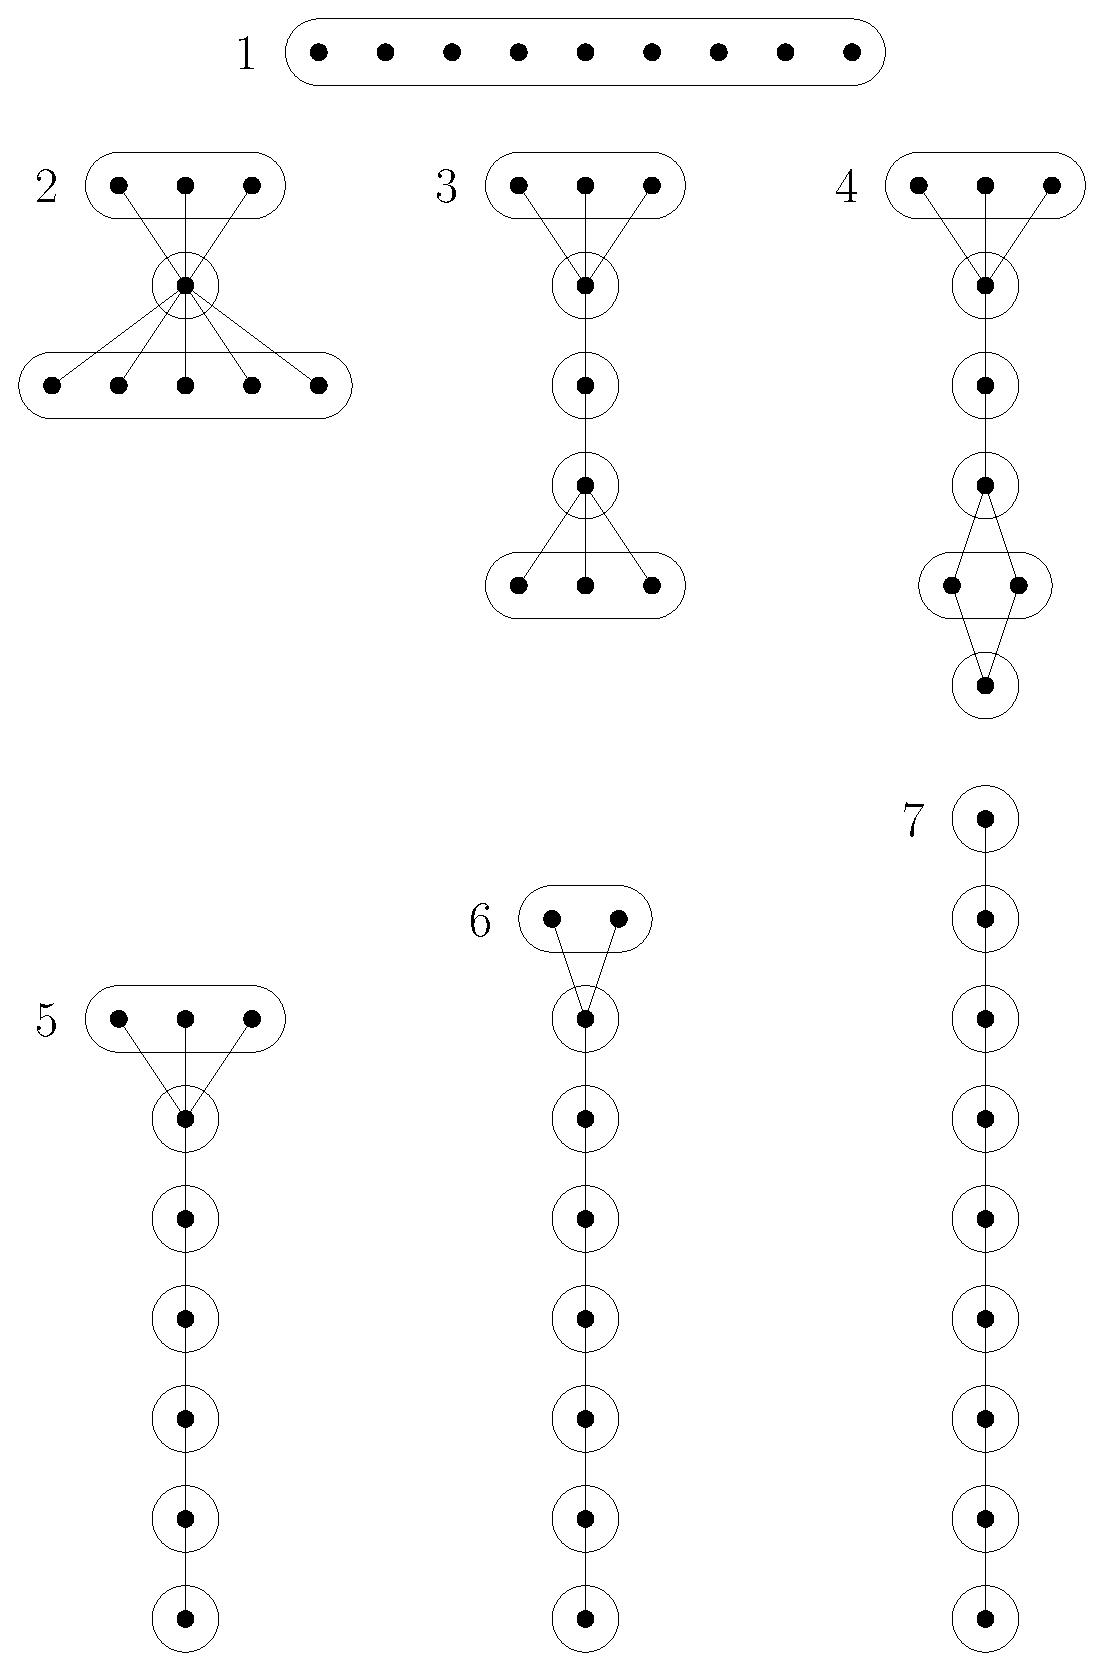
\includegraphics[width=\textwidth]{fig/supi/quicksort}} \caption{Steps of the
\quicksort algorithm represented as Hasse diagrams (maximal antichains / stable
sets are circled).} \label{fig:supi:quicksort} \end{subfigure}
~
\begin{subfigure}[t]{0.4\textwidth}
{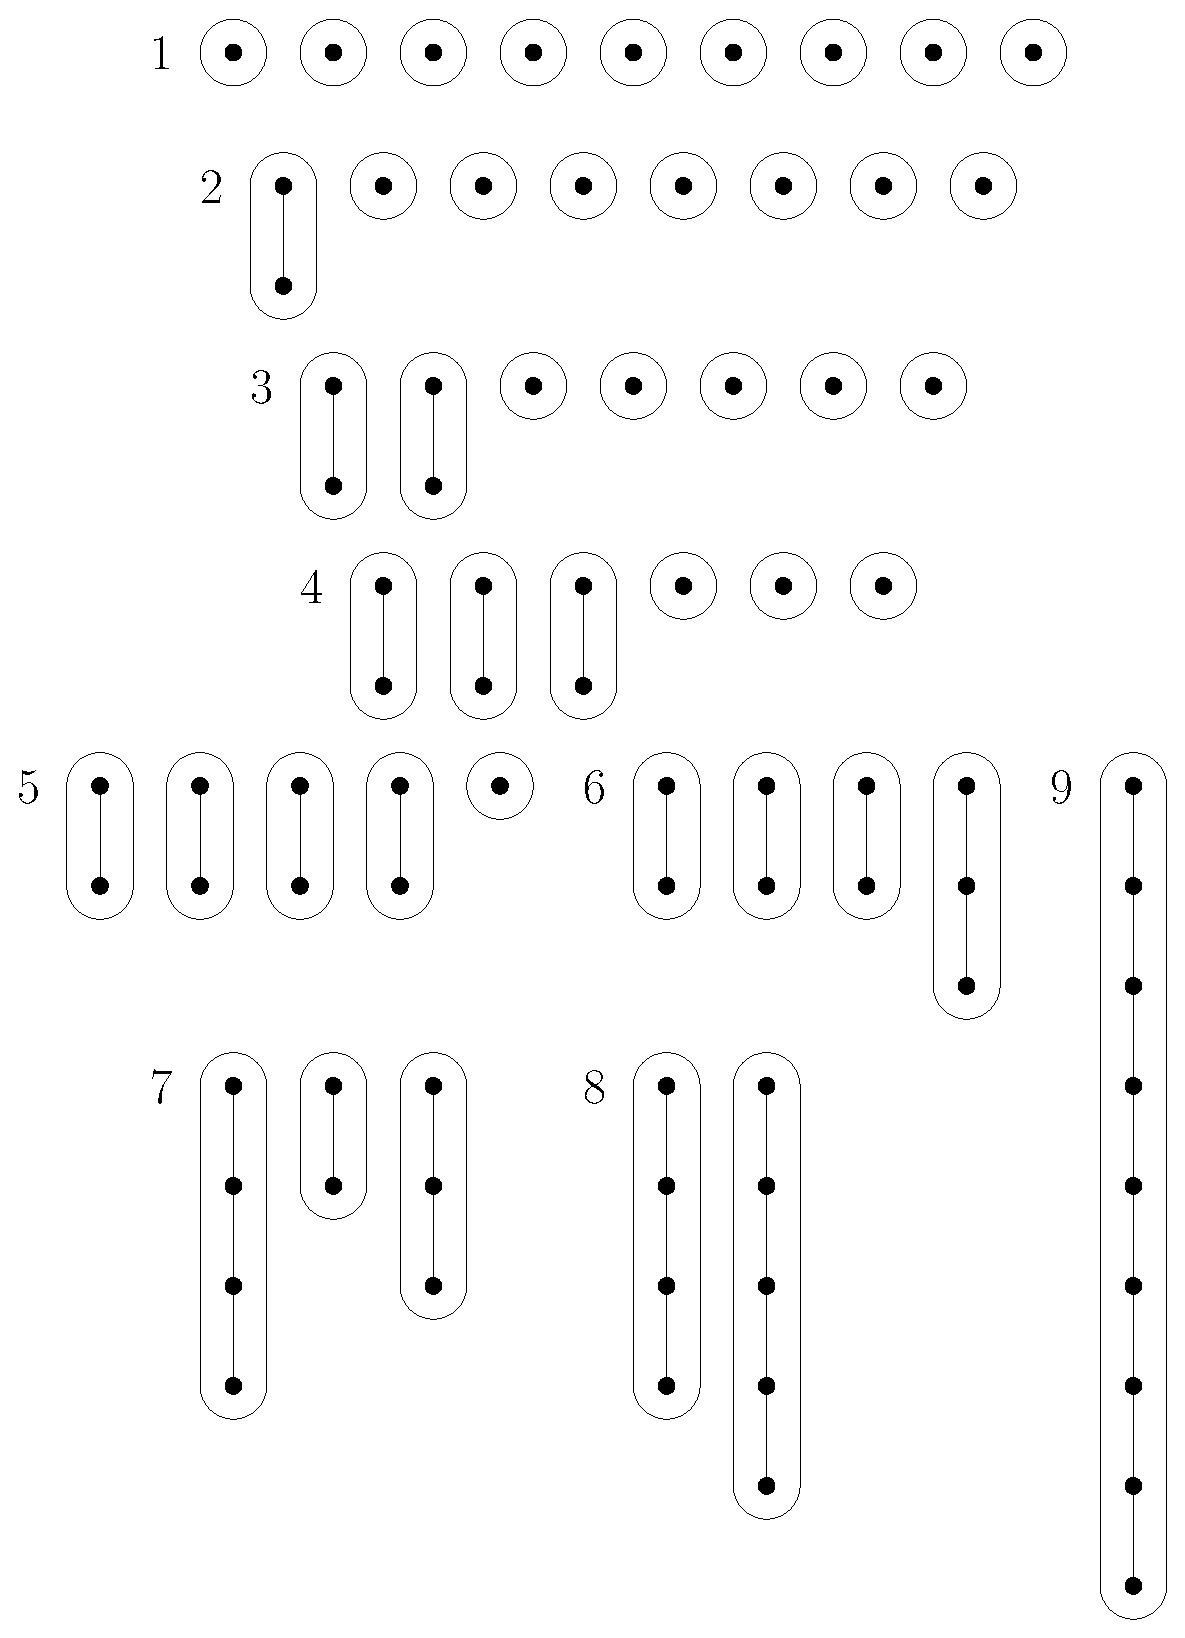
\includegraphics[width=\textwidth]{fig/supi/mergesort}} \caption{Steps of the
\mergesort algorithm represented as Hasse diagrams (maximal chains / cliques are
circled).} \label{fig:supi:mergesort} \end{subfigure} \end{figure}


\Cref{fig:supi:quicksort,fig:supi:mergesort} show the iterative poset
generation processes of a run of \quicksort and \mergesort. They sum up what we
observed about those algorithms, that they only work on a particular subset of
posets.

What we are interested in in this chapter are algorithms that can sort any
poset, \ie not only those handled by classical sorting algorithms, optimally
with respect to the number of comparisons.
